\documentclass{article}
\usepackage{lmodern} % Latin Modern Font
\usepackage[T1]{fontenc}
\usepackage{authblk}
\usepackage{amsfonts} % \mathbb
\usepackage[margin=0.5in]{geometry}
\usepackage[utf8]{inputenc}
\usepackage{graphicx}
\usepackage[backend=biber]{biblatex}
\usepackage{amsmath}

\usepackage{algorithm}
\usepackage{algorithmic}

% \usepackage{bm} % bold & upright inside math env
% \usepackage{hyperref}
% \usepackage{hypcap}
\DeclareMathOperator{\sign}{sign}
\bibliography{bibli}
% \hypersetup{
%   colorlinks=true, 
%   allcolors=black,
%   pdfauthor={Carlos Henrique Tarjano Santos},
%   pdftitle={Robust Digital Envelope Estimation Via Geometric Properties of an Arbitrary Real Signal}
% }
\title{Envelope Estimation using Geometric Properties of a Discrete Real Signal}
\author[1]{Carlos Henrique Tarjano Santos}
\author[2]{Valdecy Pereira}
\affil[1]{(corresponding author, carlostarjano@id.uff.br) Department of Production Engineering, Universidade Federal Fluminense, Rua Passo da Pátria, 156, Campus Praia Vermelha, Bloco D - sala 309, São Domingos, Niterói, RJ, Brasil, CEP: 24.210-240}
\affil[2]{Department of Production Engineering, Universidade Federal Fluminense, Rua Passo da Pátria, 156, Campus Praia Vermelha, Bloco D - sala 309, São Domingos, Niterói, RJ, Brasil, CEP: 24.210-240}

\begin{document}

\maketitle


\begin{abstract}
% Background
Despite being an elusive concept, the temporal amplitude envelope of a signal is essential for its complete characterization, being the primary information-carrying medium in spoken voice and telecommunications, for example. Intuitively, the temporal envelope can be understood as a slow varying function that multiplies the signal, being responsible for its outer shape. 
Envelope detection techniques have applications in areas like health, sound classification and synthesis, seismology and speech recognition. 
% Problem | Objectives
Nevertheless, a general approach to digital envelope detection of signals with rich spectral content doesn't exist, as most methods involve manual intervention, in the form of filter design, smoothing, as well as other specific design choices, based on a priori knowledge of the nature of the specific waves under investigation.
To address this problem, we propose a framework that uses intrinsic characteristics of a signal to estimate its envelope, eliminating the necessity of parameter tuning.
% Methods | Procedure | Approach
The approach here described draws inspiration from geometric concepts to estimate the temporal envelope of an arbitrary signal; specifically, a new measure of discrete curvature is used to obtain the average radius of curvature of a discrete wave, that will as a threshold to identify the wave's samples that are part of the envelope, in a manner similar to the alpha-shapes approach to the identification of the concave hull of a set of points.
% Results | Findings | Product
We provide visualizations of the envelope extracted via the algorithm for various real world signals, with very diverse characteristics, such as voice, spoken and sang, and pitched and non pitched musical instruments, and discuss some approaches to assess the quality of the obtained envelopes. The algorithm compares favourably with classic envelope detection techniques based on filtering and the Hilbert Transform. A Python module, installable via the Python Package Index (PyPI), with a pure Python and a specialized C++ implementation for 64 bit Windows systems, and interactive visualizations of envelopes for a diverse range of digital waves, as well as the source code for the Python implementation, are available online.
% Conclusions | Implications
Besides the most direct applications of this work to audio classification and synthesis, we foresee impact in compression techniques and machine learning approaches to audio. The discrete curvature definition presented could also be extended to three-dimensional settings, to improve shape detection algorithms based on alpha-shapes.
\end{abstract}

{\bf Keywords:} DSP, alpha-shapes, envelope detection, discrete curvature estimation, demodulation


\section{Introduction}
Envelope detection, also known as demodulation, is ubiquitous in both analogue and digital signal processing \parencite{2011CaetanoImproved}. Nevertheless, the literature in this area is very fragmented \parencite{2017LyonsDigital}. Besides, most envelope detection techniques are designed to account for very specific settings, like pure sinusoids with moderate noise content, a limitation that excludes most physical signals, as is the case of recorded sound, for example; that limitation arises in part due to the lack of a strict mathematical definition of a temporal envelope \parencite{2013Mengempirical}.

In many contexts, however, the temporal amplitude envelope of a signal plays a prominent role: according to \textcite{2017QiRelative}, for example, the envelope is at least as important as the fine structure of a sound wave in the context of the intelligibility of Mandarin tones. This is also the case for the English language \parencite{1995ShannonSpeech}, where even envelopes modulating mostly noise were still capable of conveying meaning. 

The envelope also helps to impart emotion and identity to the human voice \parencite{2018ZhuContributions}, and envelope preserving characteristics in concert halls are associated with their pleasantness \parencite{2011LokkiEngaging}.

When dealing with broadband signals, approaches tailored to specific applications are prevalent, such as the one presented by \textcite{2014YangFast} for the distributed monitoring of fibre optic or the one formulated by \textcite{2018AssefModeling} in the context of medical ultrasound imaging.

The problem of envelope detection, normally associated with the field of digital signal processing, can be made equivalent to the geometric problem of defining the (outer) shape of a set of points in $ \mathbb{R}^2 $, provided a method for addressing the difference of units in the horizontal, time related, and vertical, amplitude related, axes of a digital signal is available, rendering the original DSP problem readily approachable via geometric techniques.

One direct way of defining the shape of a set of points in $ \mathbb{R}^2 $ is using the convex hull: as defined in \textcite{2008BergComputational}, the convex hull of a set of points $ S $ in two dimensional space is the smallest convex subset of the plane that contains all the points in $ S $. Convex hulls are unique, in the sense that a set of points define one and only one convex hull.

Generalizing that definition, \textcite{1983Edelsbrunnershape} introduced the concept of alpha-shapes, that can be seen as a Concave Hull; a mathematically well-defined generalization of the Convex Hull of a finite set of points, closely related to the Delaunay triangulation and Voronoi diagrams of those points. 

The intuition behind the alpha shapes algorithm as that only points that can be touched by a circle of radius $ \alpha $ coming from an infinite distance towards the set of points of interest are part of the frontier, that is, of the Concave Hull of this set.

Once an $ \alpha $ parameter is defined alpha shapes conserve the uniqueness property, besides reducing to the Convex Hull when $ \alpha = \infty $. Consider, for example, the artificially generate discrete wave in figure \ref{fig:Hulls}
below, where the links between consecutive samples were deemphasised to highlight the "set of points" nature of a signal: The Convex Hull and a Concave Hull, in the form of an alpha shape with a particular value of $ \alpha $ are illustrated.

\begin{figure}[ht!]
  \centering
    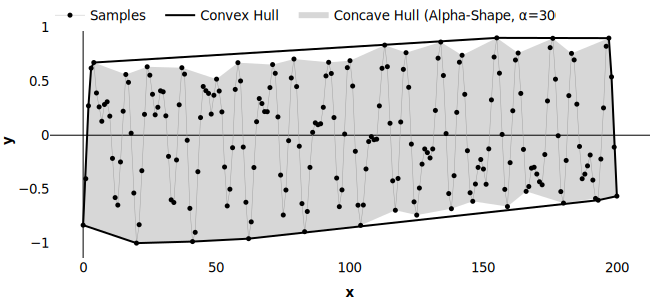
\includegraphics{images/00ConvexHull.pdf}
  \caption{A discrete signal interpreted as a set of points in the Cartesian plane, and the Convex Hull and Concave Hull at $ \alpha=300 $ defined by it}
  \label{fig:Hulls}
\end{figure}

The alpha shapes approach is used in areas such as the detection of features in images \parencite{2016VarytimidisAlpha}, reconstruction of surfaces from a cloud of points \parencite{2015WuAutomated} and Spectroscopy \parencite{2019XuModeling}, with the last work, which involves the estimation and removal of the Blaze function (a kind of envelope) of an echelle spectrograph, being particularly illustrative of the potential of synergy between geometric and DSP approaches.

Other steps in the direction of translating geometric algorithms to the context of envelope detection were also made by \textcite{2015YangSkeleton} via an algorithm based on the construction of a skeleton underlying the digital wave of interest, and also via the direct translation of computer vision methods to the task of envelope detection \parencite{2015YangRepresenting}.

Following this path, we present a general approach to envelope detection, exploiting the intrinsic characteristics of a generic, spectrally complex wave, in order to avoid as much as possible the need for manual intervention or parameter tuning, such as the choice of $ \alpha $.

% TODO <|<|<|<|<|

While the robustness of the proposed approach allows it to be used as a plug-in replacement for many methods encountered in the literature, we feel that it would be particularly useful for sound synthesis.

The envelope is shown to add complexity to the spectral representation of a wave \parencite{2019TarjanoNeuro}, and an accurate description of the envelope, while describing the evolution of the instantaneous amplitude of a signal in time, would also greatly simplify further spectral analysis. Moreover, the algorithm developed in this work naturally divides a signal into its pseudo-cycles, pinpointing them in the time domain, providing the building blocks for the reconstruction of the fine structure of the wave.

The rest of this paper is divided as follows: After explaining and defining the various entities to be used subsequently, of which the concept of frontiers is arguably the most important, in the methodology section, we dedicate a section to present a new discrete curvature estimation approach, and how it was used to identify the frontiers of a discrete wave.

We then proceed to illustrate the results of the application of the algorithm in a set of six diverse sound waves, ranging from voice to unpitched instruments comparing, afterwards, its performance with that of classic digital envelope estimation algorithms, both from a visual and numerical standpoint.

We then discuss the implications of the work, emphasizing the focus on the construction of new interpretations of the relationship between time domain and frequency domain sound descriptions, and our vision of the impact of this methodology in the field of sound synthesis, providing directions for future developments.

\section{Methodology}
% Overview of methods

\subsection{Characterization of a temporal envelope}

The interest in the theory of envelope detection arose in the analogue domain, with the widespread adoption of radio communications, where the problem is typically restricted to simple sinusoids, often with well defined frequencies \parencite{2011TurnerDemodulation}.

In this context, the most mathematically sound definition of an envelope involves the representation of its underlying wave as an analytic signal, introduced by Gabor in 1946 \parencite{2007HahnHistory}. In his work, \textcite{1946GaborTheory} applies the then relatively new mathematical machinery of the quantum mechanics to unify the time and frequency domain representations of a wave, showing how the Hilbert transform could be applied to a real signal in order to obtain an equivalent complex signal, later known as the analytic signal.

This analytic signal has the form $ A(t) = S(t) + \mathbb{H}(S(t)) \ \text{i} $ \parencite{2016HePraat} where $ S(t) $ is the original real signal. $ \mathbb{H}(S(t)) $, the Hilbert transform of the original signal, becomes the imaginary part of the analytic signal; the envelope of a signal thus represented can be straightforwardly obtained by the computation of the complex modulus of $ \mathbb{H}(S(t)) $.

Despite its widespread use, and effectiveness in the context of narrowband signals, envelope detection techniques based on the Hilbert transform don't behave well for broadband signals \parencite{2012DauSpeech}, being even physically
paradoxical in some cases \parencite{1996Loughlinamplitude}.

Figure \ref{fig:AnalyticSignal} exemplifies that, showing the envelope obtained via the analytic signal, for a pure sinusoid with a local frequency of 20 cycles, modulated by a polynomial of the third degree, illustrating the difference in the shape of the envelope in the presence and absence of Gaussian white noise with standard deviation of $ 1/10 $ of the wave's maximum amplitude.

It is readily noticeable from figure \ref{fig:AnalyticSignal} that, as soon as noise is introduced in the original signal, it is reflected in the envelope.

\begin{figure}[ht!]
  \centering
    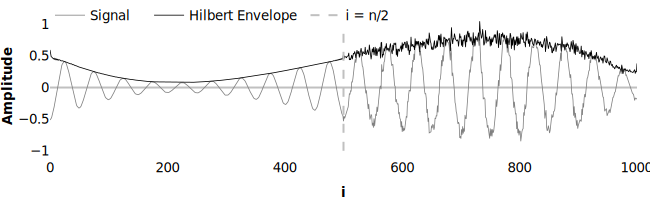
\includegraphics{images/01AnalyticSignal.pdf}
  \caption{Envelope of a pure sinusoid modulated by a polynomial of degree 3, as obtained by the Hilbert Transform approach. In the first half, the sinusoid is free of noise, while in the second half Gaussian noise with a standard deviation of $ 1/10 $ of the maximum amplitude of the wave was added to the base signal.}
  \label{fig:AnalyticSignal}
\end{figure}

In general, the problem of envelope detection, or demodulation, can be interpreted as the task of, given a continuous wave $ W(t) $, decomposing it in two components $ E(t) $ and $ C(t) $, such that $ W(t) = E(t) C(t) $ \parencite{2011TurnerDemodulation}. 
$ E(t) $ represents the slow varying part of the wave, also known as the (temporal) envelope, modulator component, or amplitude modulation (AM) of $ W $, while $ C(t) $ models its fast varying part, called throughout the literature as its (temporal) fine structure, carrier component, or frequency modulation (FM).

In the case of broadband signals, the problem of envelope detection of an arbitrary wave is ill posed, in the sense that an infinite number of pairs of $ E(t) $ and $ C(t) $ can result in the same specific $ W(t) $ \parencite{2011TurnerDemodulation, 2013Mengempirical, 1996Loughlinamplitude}.

We address this problem by assuming $ C(t) $ normalized between $ \{-1, 1\}$. This assumption doesn't cause any loss of generality since, given an arbitrary $ C(t) $, we can obtain its normalization by dividing the function by its absolute global maximum, that is, $ \hat{C}(t) = C(t) / \max(|C(t)|) $, provided that $ \max(|C(t)|) \ne 0 $.

Also, in this work we are concerned with the discrete version of this problem: given a finite digital wave represented by the vector $ \textbf{w} \in \mathbb{R}^n $, instead of the continuous function $ W(t) $, obtaining the temporal envelope of $ \textbf{w} $. 

The preceding definitions can be translated to this discrete scenario assuming that the discrete quantities arise from observing the continuous ones at regular time intervals. In that case, the equality $ i = t \ \text{fps} $ can be used to link both settings, where $ i $ is the index of each observation, $ t $ stands for the time in seconds, and fps is the frame rate, or the number of observations made in the period of a second. We can thus define:

\begin{equation} \label{eq:Envelope}
  \begin{align}
    & \textbf{w}, \textbf{e}, \textbf{c} \in \mathbb{R}^n \\
    & \textbf{w} = (w_0, w_1, \cdots, w_{n-1}) \\
    & \textbf{e} = (e_0, e_1, \cdots, e_{n-1}) \\
    & \textbf{c} = (c_0, c_1, \cdots, c_{n-1}) \\
    & \textbf{w} = \textbf{e} \odot \textbf{c} \\
    & w_i = e_i c_i \quad \forall \quad i, 0 \le i \le n-1
  \end{align}
\end{equation}

The $ \odot $ operator in \ref{eq:Envelope} stands for the Hadamard product, denoting element wise multiplication of two vectors. Figure \ref{fig:Envelope} provides an example of the vectors just defined: \textbf{w} is obtained by modulating the normalized carrier wave \textbf{c} using the smooth envelope \textbf{e}.

Note from Figure \ref{fig:Envelope} that, at some local maxima, the envelope is defined, being in fact equal to the value of the wave \textbf{w}, since $ c_i = 1 $ at those points, rendering $ e_i = 1 w_i $. The carrier wave \textbf{c} is periodic, and normalized between $ \{-1, 1\}$. Each cycle of the wave, then, reaches the value 1 only at its maximum making $ w_i$ equal to the value of the envelope at that point.

% TODO <|<|<|<|<| we will assume that this assumption holds for quasi periodic signals: that is, the absolute maximum of each pseudo cycle is equal to the value of the envelope at that point, the other local extrema in that same cycle are the ones that should be filtered out.

% TODO <|<|<|<|<| We lack a indicator to evaluate the quality of the envelope, once one is identified, but figure suggests that, once the envelope is removed from w, the wave should then be confined between the interval $ \{-1, 1\}$.

Image \ref{fig:Envelope}, along with the Concave Hull illustrated in figure \ref{fig:Hulls}, helps forming the intuition behind the method developed in this work: the idea is to identify the local extrema that touch the envelope (or, to put in another way, the local extrema in relation to the whole wave that are global extrema inside their own pseudo cycles), filtering out those who don't; in this way, we're defining the envelope itself at those points.

In this work, this is accomplished with the use of a circle of a defined radius, large enough to prevent it from reaching the smallest local extrema when "rolled" around the (geometric) representation of the wave: only the extrema touched by the circle will be marked as part of the envelope.

In the next section such a geometric representation will be formulated, along with the necessary tool to estimate the average curvature of the wave and, consequently, the appropriate radius of the circle.

% TODO <|<|<|<|<|

\begin{figure}[ht!]
  \centering
    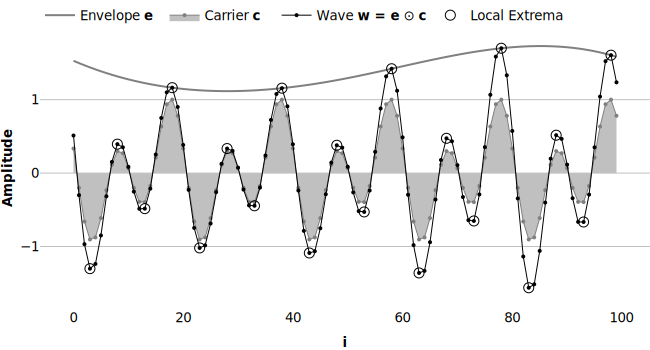
\includegraphics{images/02Envelope.pdf}
  \caption{Example of a discrete wave \textbf{w} composed by the element wise multiplication of an envelope \textbf{e} and a carrier \textbf{c}. The local extrema of \textbf{w} are highlighted with a circle.}
  \label{fig:Envelope}
\end{figure}

\subsection{Simplified Representation}

Instrumental to the method here presented is the definition of a pulse: each time the value of \textbf{w} changes sign, that is, every time the discrete wave \textbf{w} represents crosses the horizontal axis, the beginning of a pulse is defined, with the next crossing defining its end. This definition is in line with the one presented in \textcite{national1996telecommunications}, where a pulse is defined as a rapid change in the amplitude of a signal, followed by a fast return to the baseline value; zero, in our case.

From \ref{fig:Envelope} we can see that only the maximum point of a positive pulse or the minimum point of a negative one can potentially be equal to the envelope and are, thus, our only points of interest. We can then proceed with the rest of the method considering only those points, to great computational advantage. 

For this reason we define P as the set of the points $ \{P_0, P_1, \cdots, P_{m-1}\} $ where $ P_j = (i_j, \lvert w_j \lvert) $, that is, $ \lvert w_j \lvert $, the absolute value of the extrema of each pulse, becomes the ordinate of each point and $ i_j $, its original index, becomes the abscissa.

This relation is illustrated in figure \ref{fig:Pulses}. We call it P to emphasize the connection with the pulses of \textbf{w}, noting that P is, in fact, a set of points.

\begin{figure}[ht!]
  \centering
    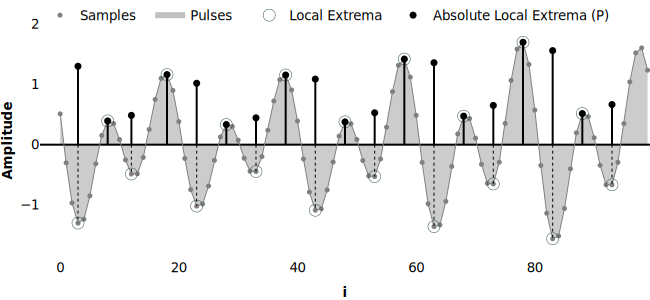
\includegraphics{images/03Pulses.pdf}
  \caption{Example of a discrete wave \textbf{w} divided into pulses, of which the extrema are highlighted with a circle. P is the set of the points $ P_j = (i_j, \lvert w_j \lvert) $ representing the absolute value of those extrema.}
  \label{fig:Pulses}
\end{figure}

P is not fit for geometric interpretation yet, since the abscissa and ordinate of his orthogonal coordinate system have different units: in the vertical axis we have a unit related to the instantaneous intensity of the wave, while in the horizontal axis we have the index at which each extremum occurs, ultimately a time related unit. 

Specifically, this coordinate system has a basis vector $ \mathbf{b} = \{ \mathbf{b}_x, \mathbf{b}_y \}$ with $ \mathbf{b}_x = (a, 0), \mathbf{b}_y = (0, i) $ where $ a $ is an amplitude unit such as decibel, a measure of the instantaneous sound pressure, volt or even a fraction of a fixed maximum value. $ i $ represents the index of the sample, and is linked to time by the aforementioned relation $ i = t \ \text{fps} $.

We are interested in finding a coordinate system where a pulse's amplitude $ \lvert w_j \lvert $ and length would define, in average, a square. 

To achieve that, we divide the basis vector of the original vertical axis by the average of all ordinates, effectively cancelling the unit of the vertical components of the points. We could divide the basis vector of the horizontal axis by the average of the difference between the abscissa of a point and the abscissa of the immediately posterior, likewise eliminating the axis' unit. 

The drawback is that we would lose the direct link between P and \textbf{w} that arises from the fact that the abscissas of the points in P are indices $ i $ of \textbf{w}: we choose instead to leave the abscissa intact and multiply the now unitless vertical basis axis by the average of the difference between the abscissa of a point and the abscissa of the immediately posterior. In this way, both axes will have unit $ i $, and the relation is preserved, making it easier to recover the envelope points later.

In this new coordinate system we have a basis vector $ \mathbf{b}^\prime = \{ \mathbf{b}^\prime_x, \mathbf{b}^\prime_y \}$ where $ \mathbf{b}^\prime_x = (i, 0) $ and $\mathbf{b}^\prime_y = (0, i) $, related to the original basis vector by:

\begin{equation} \label{eq:Basis}
\begin{align}
\mathbf{b}^\prime_x &= \mathbf{b}_x  \\
\mathbf{b}^\prime_y &= \frac{\left( \frac{i_{m-1} - i_0}{m-1} \right)}{\left( \frac{\sum_{j=0}^{m-1} \lvert w_j \lvert}{m} \right)} \mathbf{b}_y 
\end{align}
\end{equation}

The effect of this normalization can be seen in the points shown in figure \ref{fig:Vectors}, shown in scale in both coordinate systems. The set V of the vectors from each point of P to the next is also shown in the picture, as it will be used to estimate the average curvature of P, we define this set below.

\begin{equation} \label{eq:Vectors}
\begin{align}
\text{V} = \{ v_0, v_1, v_{m-2} \} \quad \text{where} \quad v_k = P_{j+1} - P_j \quad \forall \quad 0 \le k \le m-2
\end{align}
\end{equation}

\begin{figure}[ht!]
  \centering
    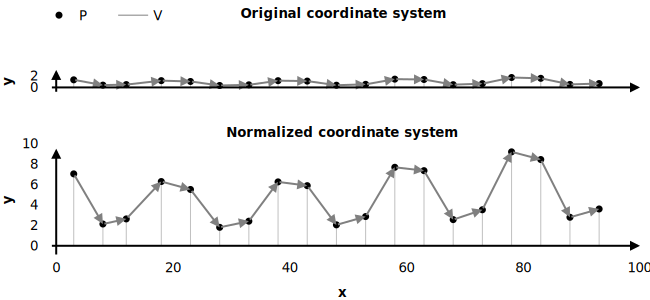
\includegraphics{images/04Vectors.pdf}
  \caption{The set of points P and the set V of vectors between two adjacent points of P, in both the original and normalized coordinate systems, shown in scale.}
  \label{fig:Vectors}
\end{figure}

\subsection{Discrete Curvature Estimation}

Translating the explanation of alpha-shapes in \textcite{1994EdelsbrunnerThree} to our context, we can say that the points that are part of the envelope are those touched by a circle of a given radius $ r $, coming from $ y \to \infty $ towards the signal, that is not allowed to contain any point of the signal. % TODO refine

Intuitively, one can picture a circle being rolled above the signal, and marking the points it touches as envelope points.

To infer the appropriate radius $ r $ of such circle a measure of discrete curvature is needed. Discrete curvature estimation is an important task in image processing \parencite{2010FleischmannNovel} for which no default definition exists. 

The two possible general approaches are the derivation of direct methods, that use characteristics of the discrete wave to calculate the curvature, or the use of the curvature of a smooth, continuous curve fitted to the discrete wave \parencite{2001CoeurjollyDiscrete}.

% Concerning the last method, two approaches to fit a polynomial to a generic wave are readily available: the least mean squares approach, that seeks to minimize the dependent variable errors and the total least squares problem, that treats both variables symmetrically \parencite{1980GolubAnalysis}.

% The geometric, symmetrical nature of the problem excludes the more computationally economic least mean squares approach, however, leaving us with the total least squares, for which no general closed-form solutions are available \parencite{2007MarkovskyOverview}; this leads us to turn our attention to direct approaches of curvature estimation.

Concerning direct methods \textcite{2014CarrollSurvey}, for example, derive three such definitions based on the approximation of a circle by an inscribed, centred and circumscribed polygon. In the context of tridimentional meshes, \textcite{2016VasaMultivariate} evaluate a range of existing estimators from a multivariate point of view.

Those approaches define the discrete curvature in relation to the vertices of a wave. In our particular case, it wouldn't make sense to talk about the curvature of a single pulse, since it is what our points ultimately represent. Instead, we are interested in the change of direction, what the term curvature ultimately means, between two adjacent pulses, as the vectors in the set V suggests.

We thus proceed to define a discrete curvature measure over the edges of a discrete wave. To that end we are going to apply the definition of smooth curvature as the rate of change of the unit tangent to a curve, noting that this is equivalent to that of the osculating circle \parencite{2016VasaMesh}.

\subsubsection{The Equivalent Circle Approach}

The rationale is to find, for each vector $ v_k \in \text{V} $, the radius $ r_k $ of the equivalent circle whose tangent has the same change in direction, in the same horizontal distance, as the vector of interest, as shown in figure \ref{fig:DiscreteCurvature}. The average curvature of the P will then be obtained by the average of all radii $ r_k $.

\begin{figure}[ht!]
  \centering
    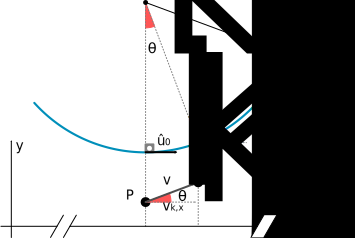
\includegraphics{images/05DiscreteCurvature.pdf}
  \caption{The tangent unit vector of the circle changes from the horizontal direction in $ \hat{u}_0 $ to an inclination of $ \theta $ in $ \hat{u}_1 $, $ \theta $ being the angle that the vector $ v_k $ makes with the horizontal direction.}
  \label{fig:DiscreteCurvature}
\end{figure}

From figure \ref{fig:DiscreteCurvature} is easy to see that $ r_k = v_{k,x} \sin(\theta_k)$ where $ v_{k,x} $ is the component of $ v_k $ in the horizontal direction; $ \theta_k $ itself can be obtained using the slope $ m_0 = 0 $ of any line in the horizontal direction and the slope $ m_k = v_{k,y} / v_{k,x} $ defined by $ v_k $ via the equality $ \theta_j = \arctan \big( (m_k - m_0) / (1 + m_k m_0) \big) $.

The radius of the circle that represents the average curvature of V, and will be used to obtain the envelope of the discrete wave \textbf{w} can be obtained via equation \ref{eq:Radius}:

\begin{equation} \label{eq:Radius}
% \begin{gather}
r = \frac{\sum\limits_{k=0}^{m-2} \left( \frac{v_{k,x} \sqrt{v_{k,x}^2 + v_{k,y}^2}}{ v_{k,y}} \right)}{m-2}
% \end{gather}
\end{equation}

We need now to construct an algorithm, using the radius just obtained, to identify the points that belong to the envelope.
Generally, the algorithm for the alpha-shapes approach resorts to the construction of the Delaunay triangulation of the set of points, that is latter filtered. We can adopt a more straightforward method, as our points have a defined structure:

Let $ x_o, y_o \in \mathbb{R}, \quad 0 \le y_o < +\infty $ be the coordinates of the center of a circle with radius $ r $, that can be placed anywhere in the upper plane of the coordinate system;

Let $ P_a, P_b, P_c \in \text{P}, \quad P_a \ne P_b \ne P_c $ be three different points of the set P;

For all circles of center $ x_o, y_o $ and radius $ r $ that can be constructed to pass through any two different points of P, that is, $ \forall \quad P_b, P_c $ such that $ (P_{b,x} - x_o)^2 + (P_{b,y} - y_o)^2 = (P_{c,x} - x_o)^2 + (P_{c,y} - y_o)^2 = r^2 $, $ P_a $ will be part of the set $ E $ of the points belonging to the envelope if and only if none of those circles contain $ P_a $, or $ P_a \in \text{E} \leftrightarrow (P_{b,x} - x_o)^2 + (P_{b,y} - y_o)^2 > r^2 $. Formalizing, we have:

\begin{equation} \label{eq:InEnvelope}
\begin{align}
& P_a \in \text{E} \leftrightarrow (P_{b,x} - x_o)^2 + (P_{b,y} - y_o)^2 > r^2, \\
& \forall \ P_b, P_c \mid (P_{b,x} - x_o)^2 + (P_{b,y} - y_o)^2 = (P_{c,x} - x_o)^2 + (P_{c,y} - y_o)^2 = r^2, \\
& P_a, P_b, P_c \in \text{P}, \quad P_a \ne P_b \ne P_c \quad \text{and} \quad x_o, y_o \in \mathbb{R}, \quad 0 \le y_o < +\infty
\end{align}
\end{equation}

The algorithm follows directly from the definition in \ref{eq:InEnvelope} after noting that the first and last members of P will always be part of the envelope, since they are reachable a circle of any radius $ r $. From $ P_0 $, our first pivot point, we construct circles passing through $ P_1, P_2, \cdots, P_d $ until a circle that doesn't contain any point in P is found; $ P_d $ then becomes the new pivot point and is included in E, and this procedure continues until $ P_{m-1} $ is reached.

The procedure is formalized in algorithm \ref{FindEnvelope}. We don't provide similar algorithmic descriptions of the preceding steps since the Python implementation can easily serve as pseudocode.

\begin{algorithm}[H]
\caption{Retrieve Envelope} \label{FindEnvelope}
\begin{algorithmic}
\STATE \textbf{Given} $ \text{P} = \{P_0, P_1, \cdots, P_{m-1}\}, r $, \textbf{circle}, a function that returns the center of a circle of a given radius passing through two points and \textbf{distance}, a function that returns the Euclidean distance between two points,
\STATE \textbf{Let} $ \text{E} = \{ P_0 \}, \text{id1} = 0, \text{id2} = 1 $
\STATE \textbf{Define} $ P_c = \text{point}, \text{empty} = \text{boolean} $
\WHILE {$ \text{id2} < m $}
  \STATE $ P_c \leftarrow \textbf{circle}(r, P_\text{id1}, P_\text{id2}) $
  \STATE empty $ \leftarrow $ \TRUE 
  \FOR{$ i = \text{id2} + 1 $ \TO $ m $}
    \IF {$ \textbf{distance}(P_c, P_i) < r $}
      \STATE empty $ \leftarrow $ \FALSE
      \STATE id2 $ \leftarrow \text{id2} + 1 $
      \STATE \textbf{break}
    \ENDIF
  \ENDFOR
  \IF {empty}
    \STATE E $ \leftarrow $ E $ \cup \ \{ P_\text{id2} \} $
    \STATE id1 $ \leftarrow $ id2
    \STATE id2 $ \leftarrow \text{id2} + 1 $
  \ENDIF
\ENDWHILE
\end{algorithmic}
\end{algorithm}

The set E obtained via algorithm \ref{FindEnvelope} is a set of points. The most straightforward way to transform those points into the vector $ \textbf{e} \in \mathbb{R}^n $ is via linear interpolation, the approach used in this work. 
is worthy noting, however, that many other procedures are available, both for the interpolation and the smooth approximation of points. We deliberately choose linear interpolation to avoid blurrying the results of the method.

\section{Results}
% Revisit purpose and methods
% Overview of results

\subsection{Quality of an envelope}

There are no agreed upon objective metrics to assess the quality of an envelope. Recalling figure \ref{fig:Envelope}, however, and the accompanying discussion, an intuitive way is to consider the carrier wave \textbf{c}, and how well it seems to be bounded in amplitude in the interval $ \{-1, 1\} $. To that end, with provide the follow figures of original discrete waves \textbf{w}, their envelope \textbf{e}, and the inferred carrier, obtained after dividing, element wise, the original wave by its envelope.

\begin{figure}[ht!]
  \centering
    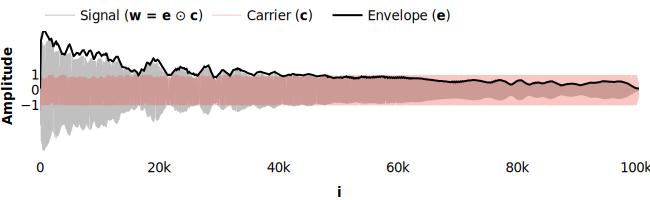
\includegraphics{images/06Graph_bend.pdf}
  \caption{Signal, envelope and carrier for a record of a bend performed on an electric guitar.}
  \label{fig:Bend}
\end{figure}




Due to an assortment of factors, such as the unconventional approach presented in this work and the intrinsic dificult in visualizing discrete waves given their high dimensionality, the authors deemed helpful to provide a companion website with interactive visualizations.

An implementation of the method in pure Python, fully functional, can also be found at the repository dedicated to this work as well as a Python module available at the Python Package Index (PyPI) and conveniently instalabbe via the command `pip install signal-envelope`. Besides, those working under Windows 64 bit can benefit from a specialized dll coded in C++ that is automatically used within this module.



In an effort to formalize the assessment of the quality of temporal envelopes, \textcite{1996Loughlinamplitude} proposed some conditions necessary, but not sufficient, to ensure the physical plausibility of an envelope. We comment briefly below that the algorithm here presented satisfies the four conditions presented.

The first one states that if a signal is bounded in magnitude, then its envelope should be, as well. Our algorithm complies with this requisite, as the envelope is composed of selected samples from the original signal itself;

The second statement is that if the signal has a finite frequency range, that frequency range must not be exceeded by the envelope. This is only directly applicable in the continuous case, where this condition was proposed.

Nevertheless, if we picture both the wave and the envelope as samples from continuous functions, is easy to see that this t is the case for our algorithm; since the envelope is composed by some samples of the digital wave, in the limit where all the samples of the wave are also part of the envelope, we have that the maximum frequency for both is the same. 

In all other cases, the maximum frequency of the envelope will be smaller than that of the original wave. The range of frequencies of the envelope, then, will always lie between zero and the maximum frequency of the original wave.

The third condition states what, for a periodic signal, the envelope should be a straight line with the intercept equal to the amplitude of this signal. Since all the local maxima have the same amplitude, our envelope will indeed be a straight line, with the same amplitude as the original wave.

The fourth and last condition states that if a wave is multiplied by a constant, the envelope should also be multiplied by the same constant. That is also the case, again because the points that form the envelope are points of the original wave itself.

\subsection{Comparison with traditional algorithms}

Direct comparison with many of the more recent algorithms is made difficult by the unavailability of digital implementations of such works, many designed to process analogue signals \parencite[e.g.,][]{2018AssefModeling}.

Nevertheless, insight can be gained from a comparison of the results of the method here proposed with some of the most common envelope extraction algorithms, as can be seen in figure \ref{fig:Comparison}.

\begin{figure}[ht!]
  \centering
    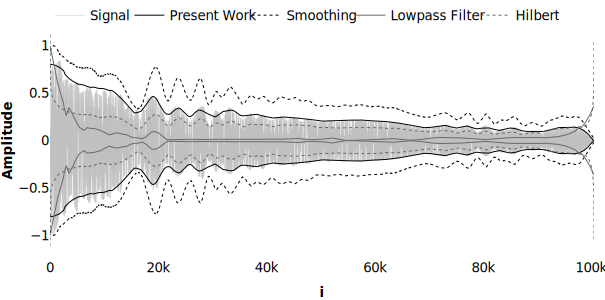
\includegraphics[width=0.8\linewidth]{12Comparison.pdf}
  \caption{Comparison of the algorithm present in this work with the most common methods of digital envelope identification.}
  \label{fig:Comparison}
\end{figure}

For a recording of a guitar sound, in which a bend is performed, we contrast the proposed algorithm with four common approaches of varying complexity: simple smoothing of the rectified original wave, low pass filtering followed by rectification, peak identification and subsequent smoothing, and the extraction of the envelope via Hilbert transform, as presented earlier in the paper, with a previous smoothing of the original wave to avoid the artifacts shown in figure \ref{fig:AnalyticSignal}.

All those methods demanded careful choice of parameters: in the case of filtering, a cut-off frequency of approximately 88 Hz was used, consisting of one additional parameter to be tuned. For all the other traditional approaches, the Savitzky-Golay smoothing algorithm was used, and the window size was the parameter to be defined.

In the case of the proposed algorithm, the smooth temporal envelope was obtained merging both positive and negative frontiers, the result being smoothed with the same procedure described. Figure \ref{fig:FrontiersToEnvelope} illustrates the results.

\begin{figure}[ht!]
  \centering
    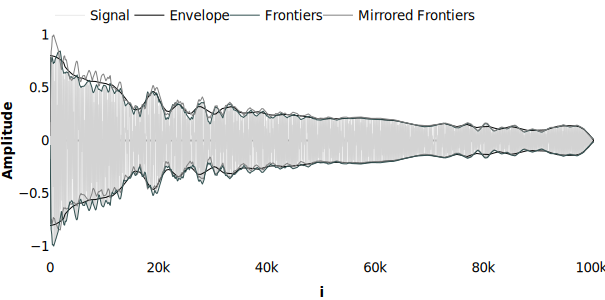
\includegraphics[width=0.8\linewidth]{13FrontiersToEnvelope.pdf}
  \caption{Original positive and negative frontiers in dark grey and their mirrored versions. The temporal envelope, in black, is obtained by merging and approximating both frontiers.}
  \label{fig:FrontiersToEnvelope}
\end{figure}

Table \ref{table:Comparison} presents a computational comparison between the techniques. The times are for custom implementations of those methods in the Python programming language. The least mean squares result was calculated by halving the envelopes presented in figure \ref{fig:Comparison} and comparing them with the rectified absolute wave, so as to avoid the potential influence of an estimated frequency. 

We can see that, while the algorithm here presented is the most accurate, it's also the most computationally intensive. The connection between alpha-shapes and Delaunay triangulation can be explored in future works as a means to improve the efficiency of the algorithm.

\begin{table}[ht!]
\centering
\begin{tabular}{ l c c }
\hline
Method & LMS & time(s) \\
\hline
Presented Algorithm & 0.0088 & 4.1507 \\ 
Smoothing           & 0.0123 & 0.1911 \\ 
Low pass Filter      & 0.0258 & 0.5601 \\ 
Hilbert Transform   & 0.0141 & 0.2599 \\ 
\hline
\end{tabular}
\caption{Comparison of the algorithm present in this work with the most common methods of digital envelope identification.}
\label{table:Comparison}
\end{table}

% \subsection{Retrieving information about the underlying wave}

% The algorithm provides the position of the pseudo-cycles of a wave, with which one can, for example, derive its fundamental frequency and phase: using one of the two frontiers, we have $ f = (\#F^\pm - 1) n / (F^\pm[-1] - F^\pm[0])$, where $ \#F^\pm $ denotes the cardinality of the frontier, while $ F^\pm[0] $ and $ F^\pm[-1] $ stand for the frontier's first and last item, respectively.

% Similarly, each point of each of the frontiers can be used to estimate the local phase at that location. For the positive frontier, it is necessary to note that, for each point, the following equation holds: $ \cos(\phi + 2 \pi f i / n) = 1 $, and thus $ \phi = 2 \pi k - 2 \pi f i / n $, with $ k \in \mathbb{N} $, while for the negative frontier $ \cos(\phi + 2 \pi f i / n) = -1 $ and $ \phi = 2 \pi k + \pi - 2 \pi f i / n) $.

\subsection{Frontiers}

In practice, is not uncommon for a discrete wave, especially in the case of sound, to present somewhat different positive and negative contours; in those cases, the algorithm here presented can be used independently in the positive and negative pulses of the wave to define two "envelopes", that we are going to call superior and inferior frontiers.

Figure \ref{fig:FullFrontiers} illustrates the frontiers of six diverse discrete sound waves, as well as an in-detail view of the highlighted segment for each signal. All waves are records of physical sounds, chosen to represent the applicability of the algorithm in real-world scenarios.

\begin{figure}[ht!]
  \centering
    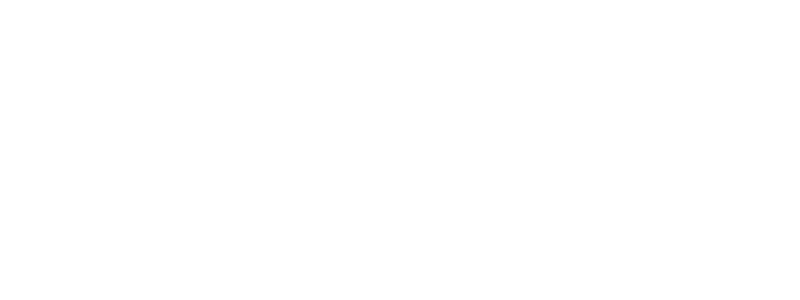
\includegraphics{images/07FullFrontiers.pdf}
  \caption{Positive and negative frontiers of six digital waves, as extracted by the algorithm here presented. For each wave, the region highlighted in black is shown in detail besides the whole wave. For each wave the horizontal axis is the sample number $i$, while the vertical axis is the normalized amplitude. All 6 waves were recorded at 44100 fps.}
  \label{fig:FullFrontiers}
\end{figure}

The frontiers are satisfactorily detected in the case of harmonic and inharmonic sounds, and is robust in relation to the number of samples and the frequencies of the waves.


% The impact of the normalization of a wave using the frontiers obtained can be seen in figure \ref{fig:Fourier}, which shows the original and normalized wave in the case of a recording of the key 33 of a piano both in the time and frequency domains. We can see that the Fourier power spectra is greatly simplified in the case of the normalized wave.

% \begin{figure}[ht!]
%   \centering
%     \includegraphics[width=0.8\linewidth]{08Fourier.pdf}
%   \caption{Original and normalized views of a recording of key 33 (F3, 175 Hz) from a grand piano both in time and frequency domains.}
%   \label{fig:Fourier}
% \end{figure}

% \subsection{Robustness}

% Figures \ref{fig:xRobustness} and \ref{fig:yRobustness} illustrate the computational resilience of the algorithm for scaling in both the abscissa and ordinate axes, respectively. This is due to the normalization scheme presented in equation \ref{eq:scale}.

% Although important from a theoretical standpoint, this step has an especial computational relevance in the case of digital sound waves, as they tend to be composed of a high number of samples with relatively low amplitudes, generally normalized between -1 and 1, leading to a numerical disparity between axes.

% \begin{figure}[ht!]
%   \centering
%     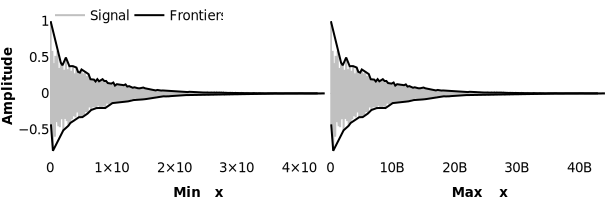
\includegraphics[width=0.8\linewidth]{10xRobustness.pdf}
%   \caption{Minimum and maximum scales of the abscissa before computational stability issues arose, for a recording of a drum kit tom.  $ \text{B} = 10^6 $.}
%   \label{fig:xRobustness}
% \end{figure}

% \begin{figure}[ht!]
%   \centering
%     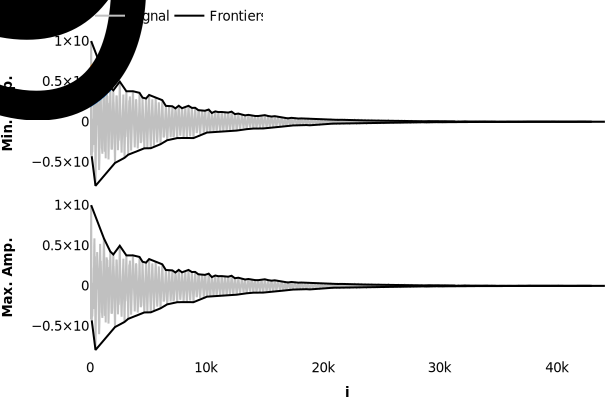
\includegraphics[width=0.8\linewidth]{09yRobustness.pdf}
%   \caption{Minimum and maximum values of the amplitude before computational stability issues arose, for a recording of a drum kit tom.}
%   \label{fig:yRobustness}
% \end{figure}




\section{Discussion}
% Put results into a broader context.

% What does it all mean?

% what principles have been established or reinforced

This work hopes to fill a gap identified by the authors in the context of sound synthesis, where the lack of procedures for the accurate identification of the temporal envelope of arbitrary waves consists of an obstacle to the complete description and eventual manipulation of signals.

While relevant in its own accord, the procedure here presented isolates the individual pseudo-cycles of a wave, pinpointing them in the time domain. Due to that, a rich set of theoretical advancements, of whose an example was given in the end of the preceding section, can be built upon this initial algorithm.

With the knowledge of the exact position and characteristics of the pseudo-cycles of a wave, one can investigate its evolution in time, in terms of waveform, for example, free from the potential interference of a modulating wave; in other words, one can have a very satisfactory view of the instantaneous shape and phase of an arbitrary wave and its evolution in time, providing a way to bridge the gap between time domain and frequency domain interpretations.

In the context of sound synthesis, for example, one would be able to apply specific methods for the recreation of the envelope, more in line with its smooth, slow varying and non-periodic nature and a different approach to the periodic and relatively fast changes of the temporal fine structure.


\subsection{Conclusion}

It is our opinion that such theoretical advances can be used in the formulation of better representations of discrete sounds, that in turn can improve sound compression techniques, while providing more adequate representation for the application of machine learning techniques for both sound classification and synthesis.

\section{References}

\printbibliography[heading=none]

\end{document}
